\part{Introduction}
%%%%%%%%%%%%%%%%%%%%%%%%%%%%%%%%%%%%%%%%%%%%%%%%%%%%%%%%%%%%%%%%%%%%%%%%%
% Introduction                                                          %
%%%%%%%%%%%%%%%%%%%%%%%%%%%%%%%%%%%%%%%%%%%%%%%%%%%%%%%%%%%%%%%%%%%%%%%%%
\section{Notes}
All mathematics notation will follow the notation used by \cite{Goodfellow-et-al-2016}. The sources of figures appear as footnotes, all other sources are found in the references section. I worked on five projects, chapters II - VI correspond to each of those projects, in chronological order.

\section{The Company}
Surewash is a small company (less than ten employees) based in the Trinity Technology and Enterprise Centre in Grand Canal Dock, Dublin, Ireland. Surewash's core focus is on designing, manufacturing, and selling educational products for hand hygiene. At the core of all of their products, a camera system is used to detect if someone is washing their hands correctly or not. Hand hygiene training is achieved by a user using this machine repeatedly until they are proficient at washing their hands. This is achieved by making it progressively harder to complete a session with the machine, so on first use, the machine will provide detailed instructions on the process, and allow a lot of time to complete each part of the process, but as time goes on, these aids are removed and if a user doesn't complete a part of the process in a certain time, they will have to redo the process.

\begin{figure}[h]
    \centering
    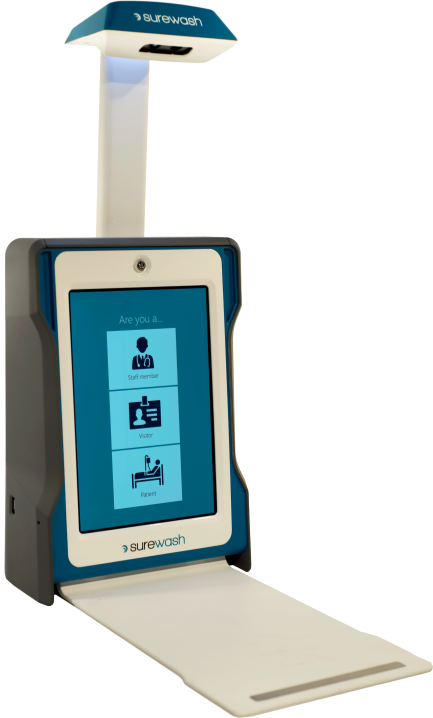
\includegraphics[height=100pt]{../img/sw_go.png}
    \space \space \space \space \space \space \space \space \space \space \space \space
    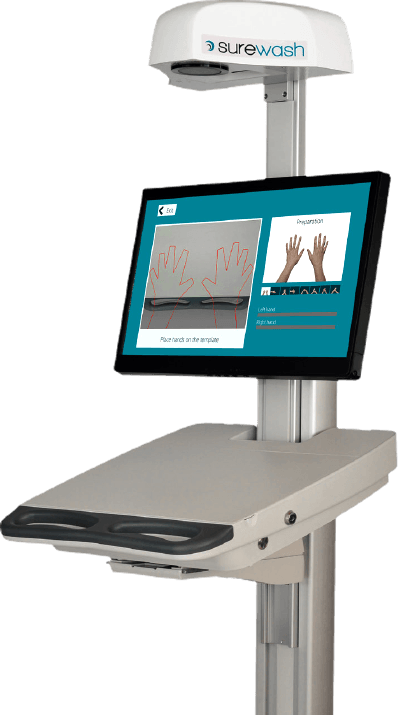
\includegraphics[height=100pt]{../img/sw_elite.png}
    \caption[]{From left to right: Surewash GO, and Surewash ELITE\footnotemark}
    \label{fig:sw_elite_go}
\end{figure}
\footnotetext{Obtained from: https://surewash.com/products/ (accessed: 30-07-2019)}

Surewash currently has three products. The Surewash ELITE, their first product, is a freestanding unit on wheels, designed to sit in a hospital ward. The Surewash GO is a smaller, and cheaper version of the ELITE. It is portable and unlike the ELITE, can be used without being connected to mains power, as long as there is sufficient charge in the battery. Its core functionality is the same otherwise, albeit in a smaller form-factor. Surewash POCKET is different to the other two products, it is a mobile app that uses a phone's front-facing camera, although it uses the same concept of levels to teach hand hygiene. The key difference with POCKET is that it cannot be used for certification of hand hygiene training since a mobile phone's camera cannot provide the same quality of data that the cameras that come with ELITE and GO can provide.

Surewash also has an online web service called Sureash.NET. Each Surewash product can upload its user data to this website and it will then display overall trends in usage to customers.

\section{My internship}
I was employed as an intern at Surewash, working normal business hours from January to July 2019. There was another intern, Gaurav Gupta.
    \subsection{Internship Goals}
    At the beginning of my internship, I set myself the following goals
        \paragraph{Improve my skills in programme design}
        Targets:
        \begin{enumerate}
            \item My company uses Python for server-side tasks.
            \item I will hone my skills in turning programme ideas into working, and understandable Python code that can be deployed on Surewash servers.
            \item I will improve my understanding of how Python works, and what is best practice.
            \item I will submit my code to my supervisor for evaluation and feedback.
        \end{enumerate}
    
        \paragraph{Enhance my time management skills}
        Targets:
        \begin{enumerate}
            \item My company uses Scrum to allocate tasks and resources, my supervisor will introduce me and help me fit into the company’s workflow.
            \item I will participate and contribute to company scrum meetings every two weeks.
            \item I will improve my ability to estimate what I can get done in a single sprint.
        \end{enumerate}

        \paragraph{Improve my presentation and public speaking skills}
        Targets:
        \begin{enumerate}
            \item I will make presentations of my work for both technical and non-technical audiences.
            \item I will receive feedback on said presentations, and use it to improve how and what I present to them.
            \item At the conclusion of my internship with Surewash, I will be confident at preparing and presenting presentations.
        \end{enumerate}